\documentclass{ximera}
\author{Jim Talamo, Jason Miller, and Bart Snapp}
\newcommand{\RR}{\mathbb R}
\renewcommand{\d}{\,d}
\newcommand{\dd}[2][]{\frac{d #1}{d #2}}
\renewcommand{\l}{\ell}
\newcommand{\ddx}{\frac{d}{dx}}
\newcommand{\dfn}{\textbf}
\newcommand{\eval}[1]{\bigg[ #1 \bigg]}


\outcome{Use reduction formulas and the Pythagorean identity to compute
  integrals involving trigonometric functions.}
\outcome{Recognize the patterns that appear in trigonometric integrals,
  and use appropriate substitutions to compute them.}
\outcome{Compute integrals involving powers of sine and cosine.}

\title[Dig-In:]{Trigonometric integrals}

\begin{document}
\begin{abstract}
  We can use substitution and trigonometric identities to find antiderivatives of certain types of
  trigonometric functions.
\end{abstract}
\maketitle

In this section, we will study how to integrate certain types of trigonometric functions.  We begin by giving the antiderivatives of the six basic trigonometric functions:


\section{Antiderivatives of other trigonometric functions}

\begin{theorem}[Antiderivatives of trigonometric functions]\hfil
  \begin{itemize}
  \item $\int \sin(x) \d x = - \cos(x)+C$
  \item $\int \cos(x) \d x = \sin(x)+C$
  \item $\int \tan(x) \d x = \ln|\sec(x)| + C$
  \item $\int \cot(x) \d x = -\ln|\csc(x)| + C$
  \item $\int \sec(x) \d x = \ln|\sec(x) + \tan(x)| + C$
  \item $\int \csc(x) \d x = -\ln|\csc(x) + \cot(x)| + C$
  \end{itemize}
\end{theorem}

We are able to establish the antiderivatives of $\sin(x)$ and $\cos(x)$ easily from the formulas for their derivatives, but how do we establish the other formulas?  

\begin{example}
Compute:

\[
\int \tan(x) \d x
\]

This can be computed with a substitution once we recognize:

\[
\int \tan(x) \d x = \int \frac{\sin(x)}{\cos(x)} \d x
\]

By setting $u = \answer[given]{\cos(x)}$, we find $\d u = \answer[given]{-\sin(x)} \d x$ and thus:

\[
\int \tan(x) \d x = \int \frac{\sin(x)}{\cos(x)} \d x =\int \answer{-  \frac{1}{u}} \d u =-\ln|u|+C = -\ln|\cos(x)|+C
\]

Using the properties of logarithms, followed by the fact that $\sec(x) = \frac{1}{\cos(x)}$ gives:

\[
-\ln|\cos(x)| = \ln \left| (\cos(x))^{-1} \right| = \ln \left| \frac{1}{\cos(x)} \right| = \ln|\sec(x)|
\]


\end{example}
 
\begin{example}
Compute 

\[ 
\int \sec(x) \d x
\]
\begin{explanation}
It may not be clear why, but let's multiply the top and bottom by $\sec(x) + \tan(x)$. 

\[
\int \sec(x) \d x= \int \sec(x) \left( \frac{ \sec(x) + \tan(x)}{\sec(x)+\tan(x)} \right) \d x = \int \frac{ \sec^{2}(x) + \sec(x)\tan(x)}{\sec(x)+\tan(x)} \d x
\]

Now we see the rationale behind multiplying top and bottom by $\sec(x) + \tan(x)$. The derivative of the denomiator of the integrand is precisely the numerator. 

If we let $u=\sec(x)+\tan(x)$ then $\d u=\sec(x)\tan(x)+\sec^{2}(x) \d x$ and thus our integral becomes

\[
\int \sec(x) \d x = \int \frac{1}{u} \d u=\ln|u|+C=\ln|\sec(x)+\tan(x)|+C
\]

\end{explanation}

\end{example}


%\begin{example}
%  Compute:
%  \[
%  \int \sec (x) \d x
%  \]
%  \begin{explanation}
%    Write with me
%    \begin{align*}
%      \int \sec(x) \d x &= \int \cos(x)^{-1} \d x\\
%      &= \int \cos^{-2}(x)\cos(x) \d x\\
%      &=\int(1-\sin^2(x))^{-1} \cos(x) \d x
%    \end{align*}
%    We have now set ourselves up for an eventual substitution:
%    \begin{center}%% used center instead of image since there is no reason for a LARGE integral in the text
%      \begin{tikzpicture}
%        \node at (0,0) {
%          $\int \underbrace{(1-\sin^2(x))^{-1}} \underbrace{\cos(x) \d x}$
%        };
%        \node at (-.6,-.7) {\small{rational function in $g$}};
%        \node at (1.4,-.7) {\small{``$\d g$''}};
%      \end{tikzpicture}
%    \end{center}
%    Set $g =\sin(x)$ so $\d g = \cos(x) \d x$, and write with me
%    \begin{align*}
%      \int(1-\sin^2(x))^{-1} \cos(x) \d x &= \int \frac{1}{1-g^2}\d g\\
%      &= \frac{1}{2}\int \frac{1}{1-g} + \frac{1}{1+g} \d g\
%    \end{align*}
%    Antidifferentiating we find
%    \begin{align*}
%      &=\frac{1}{2}\left(\ln(1-g) - \ln(1-g)\right)+C\\
%      &= \frac{1}{2}\ln\left(\frac{1+\sin(x)}{1-\sin(x)}\right)+C
%    \end{align*}
%    Note, we could stop here, but we won't because this is not the
%    typical antiderivative of $\sec(x)$. Please keep writing with me
%    \begin{align*}
%      \frac{1}{2}\ln\left(\frac{1+\sin(x)}{1-\sin(x)}\right)+C &= \frac{1}{2}\ln\left(\frac{(1+\sin(x))^2}{1-\sin^2(x)}\right)+C \\
%      &= \frac{1}{2}\ln\left(\frac{(1+\sin(x))^2}{\cos^2(x)}\right)+C \\
%      &= \ln\left(\frac{1+\sin(x)}{\cos(x)}\right)+C \\
%      &= \ln\left|\sec(x) + \tan(x)\right|+C \\
%    \end{align*}
%  \end{explanation}
%\end{example}

The formulas for the antiderivatives of $\csc(x)$ and $\cot(x)$ are found analogously.

\section{Integrals involving products of $\sin(x)$ and $\cos(x)$}

We begin with a simple example:

\begin{example}
Compute:

\[
\int \sin^{2}(x) \cos(x) \d x
\]

\begin{explanation}
Here we recognize that $\cos(x)$ is the derivative of $\sin(x)$ so substitution is a good method to use. Let $u=\sin(x)$. Then $\d u=\cos(x) \d x$ and: 

\[ 
\int \sin^{2}(x) \cos(x) \d x = \int u^{2} \d x=\frac{u^{3}}{3}+C=\frac{ \sin^{3}(x)}{3}+C
\]
\end{explanation}

\end{example}

In this example, we saw that a substitution was quite helpful.  Earlier, we saw that there were two common instances in which substitutions could be helpful to compute antiderivatives:

\begin{itemize}
\item Once we change variables, the remaining expressions in the old variable are part of the differential in the new one.  For instance, consider:

\[ \int 2x \cos\left(x^2\right) \d x\]
By setting $u=x^2$, $\d u = 2x \d x$, so the $2x \d x$ in the original integral is part of the new differential $\d u$ and:

\[ \int 2x \cos\left(x^2\right) \d x = \int \cos(u) \d u \]

\item Once we change variables, it is not complicated to write the remaining old variables in terms of the new one.
For instance, consider:

\[ \int 2x^3 \cos\left(x^2\right) \d x\]
By setting $u=x^2$, $\d u = 2x \d x$, so the $2x \d x$ in the original integral is part of the new differential $\d u$ and:

\[ \int 2x^3 \cos\left(x^2\right) \d x = \int x^2 \cos(u) \d u  = \int u \cos(u) \d u \]

where we have used the fact that $u=x^2$ in the last step above.  Note that we can do this last integral using integration by parts!
\end{itemize}

This highlights a strategy that we will employ in this section; try to let one of the trigonometric functions be our new variable, and express the remaining expressions easily in terms of it.

\begin{example}
Compute

\[ 
\int \sin^{4}(x) \cos^{3}(x) \d x 
\]

\begin{explanation}
Per the previous discussion, we have two options: we can let $u= \sin(x)$ or $u=\cos(x)$.  
If we let $u = \sin(x)$, we will have to reserve a copy of $\cos(x)$ for the differential. This leaves two powers of $\cos(x)$ left.   One of our fundamental trig identities, the Pythagorean identity:
\[
\cos^{2}(x) + \sin^{2}(x)=1
\]
can be used to covert between \emph{even} powers of sines and cosines, so this will be a fruitful approach:

We can use this identity to rewrite $\cos^{2}(x)=1-\sin^{2}(x)$ in our integral so that it becomes:
\[
\int \sin^{4}(x) (1-\sin^{2}(x)) \cos(x) \d x
\]
Now the same strategy we used in the first example of this section will work. We can do the substitution $u=\sin(x)$. We find $\d u= \answer[given]{\cos(x)} \d x$, so that the integral becomes:

\[ 
\int \sin^{4}(x) (1-\sin^{2}(x)) \cos(x) \d x =  \int u^{4}(1-u^{2}) \d u
\]

Finishing this integral we get 

\[ 
\int u^{4}(1-u^{2}) \d u= \int u^{4}-u^{6} \d u = \answer[given]{\frac{1}{5}u^5 - \frac{1}{7}u^7} + C =\frac{1}{5}\sin^{5}(x) - \frac{1}{7} \sin^{7}(x) + C
\]

Note that had we let $u = \cos(x)$, we will have to reserve a copy of $\sin(x)$ for the differential. This leaves three powers of $\sin(x)$ left! We certainly can use the Pythagorean identity from before to write:

\[ \sin^3(x) = \left(\sin^2(x)\right)^{3/2} = \left(1-\cos^2(x)\right)^{3/2} = (1-u^2)^{3/2} \]

If $u = \cos(x)$, we find $\d u = -\sin(x) \d x$, and from the above we can write the original integral as:

\[ 
\int \sin^{4}(x) \cos^{3}(x) \d x = \int \sin^4(x) u^3 \frac{\d u}{-\sin(x)} = -\int \sin^3(x) \cdot u^3 \d u = -\int (1-u^2)^{3/2} u^3 \d u
\]
This integral can be evaluated with another substitution $v = 1-u^2$ and some algebra, but it is certainly more time-consuming than the first approach!

\end{explanation}

\begin{remark}
As a reminder, the integrand should only display the variable of integration once the substitution has been completed; $x$ and $u$ cannot appear in the same integral in the final step since they depend on each other!  The previous example was typeset the way that it was in order to exhibit the simplification in a clear way.
\end{remark}
\end{example}

We can make a useful observation from this example. Our previous integral involved powers of $\sin(x)$ and $\cos(x)$. We peeled off a copy of the derivative of what we wanted to use for $u$.  If this leaves an even number of the other trigonometric function left, we can use the Pythagorean identity \[\cos^{2}(x)+ \sin^{2}(x) =1\] to write the remaining powers of the other trigonometric function in terms of $u$.  

In the preceding example, the power of cosine was odd, and for other examples, as long as the power of $\cos(x)$ in the original integral is odd, then we can peel off a $\cos(x)$ term to be used for $\d u$ and then let $u=\sin(x)$ to express the integral in terms of $u$.  This general approach is stated in more detail in the exercises, but for now let's try another example.

%BELOW IS NOW IN EXERCISES--I do not want to encourage procedural thinking in this section and worry that these general ideas will do that or be very confusing to students

%The above method relies on having a power of $\sin(x)$ multiplied by odd positive power of $\cos(x)$ so we can peel off a $\cos(x)$ term and convert the remaining even positive power into a power of $1-\sin^{2}(x)$. One can then substitute $u=\sin(x)$ and $\d u= \cos(x)$ to transform the integral to be in terms of $u$. 
%
%
%In general, if we are integrating a product of powers of sine and cosine, and the power
%of cosine is positive and odd, then the integral looks like
%\[
%\int \sin^n(x) \cos^{2k+1}(x) \d x
%\]
%where $k$ is some nonnegative integer. Then
%\begin{align*}
%\int \sin^n(x) \cos^{2k+1}(x) \d x &=\int \sin^n(x) (\cos^{2}(x))^k \cos(x)\d x\\
%&= \int \sin^n(x) (1-\sin^{2}(x))^k \cos(x) \d x.
%\end{align*}
%We have now set ourselves up for an eventual substitution:
%\begin{center}%      %COMMENT used center instead of image since there is no reason for a LARGE integral in the text
%  \begin{tikzpicture}
%    \node at (0,0) {
%      $\int \underbrace{( \sin^n(x) (1-\sin^{2}(x))^k} \underbrace{\cos(x) \d x}$
%        };
%    \node at (-.5,-.7) {\small{polynomial in $u$}};
%    \node at (1.8,-.7) {\small{``$\d u$''}};
%  \end{tikzpicture}
%\end{center}
%so letting $u = \sin(x)$ so $\d u =\cos(x) \d x$, we have 
%\[
%\int u^n(1-u^2)^k \d u
%\]
%which is a polynomial, and can be integrated term-by-term after
%expansion.


\begin{example}
  Compute:

  \[
  \int \sin^{5}(x) \cos^2(x) \d x
  \]

  \begin{explanation}
   
    If we try $u=\sin(x)$, we find that we need a factor of $\cos(x)$ for the differential, which leaves 1 power of $\cos(x)$ left, so using the Pythagorean identity would produce an unpleasant integral.  However, if we try $u=\cos(x)$, we find that we need a factor of $\sin(x)$ for the differential, which leaves 4 powers of $\sin(x)$ left.    We can rewrite this suggestively as:
    \begin{align*}
    \int &\sin^4(x) \cos^2(x) \sin(x) \d x \\
    &= \int (\sin^2(x))^2 \cos^2(x) \sin(x) \d x
    \end{align*}
    Now using the Pythagorean identity we can rewrite everything in
    terms of $\cos(x)$, but reserve the one power of $\sin(x)$ to help
    with the differential in an eventual variable substitution $u=\cos(x)$:
    \begin{center}%% used center instead of image since there is no reason for a LARGE integral in the text
      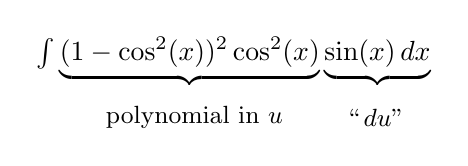
\begin{tikzpicture}
        \node at (0,0) {
          $\int \underbrace{(1-\cos^2(x))^2 \cos^2(x)} \underbrace{\sin(x) \d x}$
        };
        \node at (-.5,-.7) {\small{polynomial in $u$}};
        \node at (1.8,-.7) {\small{``$\d u$''}};
      \end{tikzpicture}
    \end{center}
    Making the substitution
    \begin{align*}
      u &= \cos(x)\\
      \d u &=\answer[given]{-\sin(x)} \d x
    \end{align*}
    yields
    \[
    \int \answer[given]{-(1-u^2)^2 u^2} \d u
    \]
    This is a polynomial in $u$, and so we can easily finish the
    integration by just expanding the polynomial out and integrating
    term-by-term. Write with me
    \begin{align*}
      \int {-(1-u^2)^2 u^2} \d u &= \int -(1-2u^2+u^4)u^2\d u\\
      &= \int-u^6 + 2u^4-u^2 \d u\\
      &=\answer[given]{-\frac{1}{7}u^7 + \frac{2}{5}u^5 -\frac{1}{3} u^3}+C
    \end{align*}
    Substituting $u = \cos(x)$ we find our final answer:
    \[
    -\frac{1}{7}\cos^7(x) + \frac{2}{5}\cos^5(x)/ - \frac{1}{3} \cos^3(x)+C
    \]
  \end{explanation}
\end{example}

Sometimes we need to massage our function into the correct form:

\begin{example}
  Compute:
  \[
  \int \sin^5(x) \d x
  \]
  \begin{explanation}
    Write with me, we start by separating a power of sine for an eventual substitution
    \begin{align*}
      \int \sin^5 x\d x &=\int \sin^4(x) \sin(x) \d x\\
      &=\int (\sin^2(x))^2 \sin(x) \d x
    \end{align*}
    Here is what we're thinking:
    \begin{center}%% used center instead of image since there is no reason for a LARGE integral in the text
      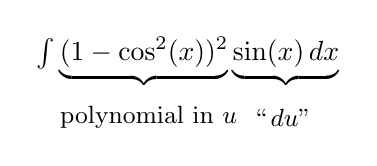
\begin{tikzpicture}
        \node at (0,0) {
          $\int \underbrace{(1-\cos^2(x))^2} \underbrace{\sin(x) \d x}$
        };
        \node at (-.5,-.7) {\small{polynomial in $u$}};
        \node at (1.2,-.7) {\small{``$\d u$''}};
      \end{tikzpicture}
    \end{center}
    Now set $u=\cos x$, $\d u=-\sin x\d x$:
    \begin{align*}
      \int \sin x (1-\cos^2 x)^2\d x&=\int \answer[given]{-(1-u^2)^2} \d u \\
      &=\int -(1-2u^2+u^4)\d u \\
      &=\answer[given]{-u+\frac{2}{3}u^3-\frac{1}{5}u^5}+C
    \end{align*}
    Hence our final answer is:
    \[
    \answer[given]{-\cos x+\frac{2}{3}\cos^3 x-\frac{1}{5}\cos^5x}+C
    \]
  \end{explanation}
\end{example}

\section{Another strategy}

Thinking again about powers of cosine and sine, what do we do when both powers are even?  Our strategy above is sunk, since peeling-off one power leaves an odd power, and we cannot use the Pythagorean identity to rewrite this in a nice way.  Instead, we will use the ``power-reduction formulas":

\begin{description}\index{power-reduction}
\item[Cosine Power-Reduction]: $\cos^2(\theta)= \frac{1}{2}+\frac{1}{2}\cos(2\theta)$ \index{cosine power-reduction}
\item[Sine Power-Reduction]: $\sin^2(\theta) = \frac{1}{2}-\frac{1}{2}\cos(2\theta)$\index{sine power-reduction}
\end{description}

\begin{question}
Using the above formula we find $\sin^2(2x) = \frac{1}{2}-\frac{1}{2} \cos(\answer{4x})$.
\end{question}

\begin{remark}
The designation ``power reduction formula" sounds quite impressive, but they result from a simple rearrangement of the double angle formula for $\cos(2\theta)$.  Indeed if we want to obtain the power reduction formula for $\cos^2(\theta)$:

\begin{align*}
\cos(2\theta) &= \cos^2(\theta)-\sin^2(\theta) \\
\cos(2\theta) &= \cos^2(\theta) - (1-\cos^2(\theta)) \\
\cos(2\theta) &= 2\cos^2(\theta)-1
\end{align*}
Solving the above equation for $\cos^2(\theta)$ gives: $\cos^2(\theta) = \frac{1}{2} +\frac{1}{2} \cos(2\theta)$.
\end{remark}

In this case, it is (usually) critical to apply the power-reduction
formulas to \textit{every} instance of cosine and sine appearing in
the integrand.

First consider a simple example:

\begin{example}
Integrate 

\[ 
\int \cos^{2}(x) \d x
\]

\begin{explanation}
The strategy of setting $u=\sin(x)$ or $u=\cos(x)$ will not produce an integral that involves an even number of the other type of trigonometric function.  Instead, we use the power reduction formula $\cos^{2}(x)=\frac{1+\cos(2x)}{2}$ to transform the integral into a form we can directly integrate.

\[
\int \cos^{2} (x) \d x= \frac{1}{2} \int 1+\cos(2x) \d x = \frac{1}{2} \left( x+ \frac{ \sin(2x)}{2} \right) + C
\]


\end{explanation}
\end{example}


\begin{example}
  Compute:
  \[
  \int \sin^2x\cos^2x\d x
  \]
  \begin{explanation} 
    The strategy of setting $u=\sin(x)$ or $u=\cos(x)$ will not produce an integral that involves an even number of the other type of trigonometric function. Use both power-reduction formulas to find:
    \[
    \int \sin^2x\cos^2x\d x=\int \left( \frac{1-\cos(2x)}{2}\right)
    \left(\frac{1+\cos(2x)}{2}\right) \d x
    \]
    From here, we can try to simplify further by multiplying out the integrand. We may end up having to
    use the power reduction formulas again to reduce the powers that appear when we multiply out the terms.  In this case
    \begin{align*}
      \int \left(\frac{1-\cos(2x)}{2}\right) \left( \frac{1+\cos(2x)}{2}\right) \d x &= \frac{1}{4} \int 1-\cos^2(2x) \d x\\
      &= \frac{1}{4} \int \sin^2(2x) \d x
    \end{align*}
    
    Since this expression has only even powers of sine, we must use
    the same strategy again, and employ a power-reduction formula:
    \[
    \sin^2(2x) = \frac{1-\cos(\answer[given]{4x})}{2}
    \]
    so we find
    \[
    \frac{1}{8}\int 1-\cos(4x) \d x = \answer[given]{\frac{1}{8}(x - \frac{1}{4}\sin(4x))} + C
    \]
  \end{explanation}
\end{example}




\subsection{Working with products of powers of $\sec(x)$ and $\tan(x)$}

The same logic used in the preceding examples can be used to find antiderivatives involving products of $\sec(x)$ and $\tan(x)$.  Indeed, the Pythagorean identity has two other forms:
\[
\sec^2(x) = 1 + \tan^2(x)  \qquad\text{and}\qquad \tan^2(x) = \sec^2(x) - 1  
\]
where the first identity we find by dividing the Pythagorean identity by
$\cos^2(x)$ and the second we find by subtracting 1 from both sides of the first identity. 

The derivatives of these functions also can be expressed in terms of each other:

\[
\ddx \left[\tan(x)\right] = \sec^2(x) \qquad\text{and}\qquad \ddx \left[\sec(x)\right] = \sec(x)\tan(x)
\]

It is worth seeing several examples where we use these identities. We proceed in a fashion similar to the procedures we saw earlier. 

\begin{example}
  Compute
  \[
  \int \tan^3(x) \sec^4(x) \d x
  \]
  \begin{explanation}
    We recall that the derivative of $\tan(x)$ is $\sec^{2}(x)$. This suggests that we might want to try $u=\tan(x)$ which requires 
    $\d u=\sec^{2}(x)$. 
    Since the power of secant is even, we can separate off a factor of $\sec^{2}(x)$ for our $\d u$. That leaves an extra factor
    of $\sec^{2}(x)$ that we must deal with. 

    \begin{align*}
    \int &\tan^3(x) \sec^4(x) \d x \\
    &= \int\tan^3(x) \sec^2(x) \sec^2(x) \d x
    \end{align*}
    Now using the identity $1+\tan^{2}(x)=\sec^{2}(x)$ we can rewrite everything in
    terms of $\tan(x)$, but reserve the one power of $\sec^2(x)$ to help
    with the differential in an eventual variable substitution $u=\tan(x)$:
    \begin{center}%% used center instead of image since there is no reason for a LARGE integral in the text
      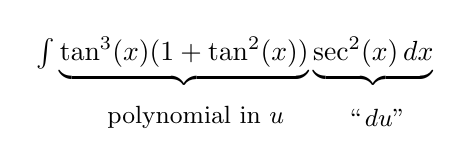
\begin{tikzpicture}
        \node at (0,0) {
          $\int \underbrace{\tan^3(x)(1+\tan^2(x))} \underbrace{\sec^2(x) \d x}$
        };
        \node at (-.5,-.7) {\small{polynomial in $u$}};
        \node at (1.8,-.7) {\small{``$\d u$''}};
      \end{tikzpicture}
    \end{center}
    Making the substitution
    \begin{align*}
       &= \tan(x)\\
      \d u &=\answer[given]{\sec^2(x)} \d x
    \end{align*}
    yields
    \[
    \int \answer[given]{u^3(1+u^2)} \d u
    \]
    This is a polynomial in $u$, and so we can easily finish the
    integration by just expanding the polynomial out and integrating
    term-by-term. We leave it to the intrepid young mathematician to
    finish this problem.
  \end{explanation}
\end{example}

%The key that was needed for success in this example was that the integrand was a products of powers of $\tan(x)$ and $\sec(x)$ where the power of $\sec(x)$ was positive and even.
%
%\[
%\int \tan^{m}(x) \sec^{2k}(x) \d x
%\]
%where $m$ is an integer and $k$ a positive integer. 
%
% This allowed us to separate off a $\sec^{2}(x)$ factor to use for the differential. 
%
%\[
%\int \tan^{m}(x)\sec^{2k-2}(x) \sec^{2}(x) \d x
%\]
%
%The remaining even power of $\sec(x)$ could be written as a power of $\sec^{2}(x)$. The identity $1+\tan^{2}(x)=\sec^{2}(x)$
%would then allow us to rewrite the remaining $\sec(x)$ factor in terms of $\tan(x)$. 
%
%\[
%\int \tan^{m}(x) ( \sec^{2}(x))^{k-1} \sec^{2}(x) \d x=\int \tan^{m}(x) (1+\tan^{2}(x))^{k-1} \sec^{2}(x) \d x
%\]
%
%Doing the substitution $u=\tan(x)$ and $\d u=\sec^{2}(x)$, our integral becomes 
%
%\[
%\int u^{m}(1+u^{2})^{k-1} \d u
%\]
%
%The integrand is a polynomial in $u$, so in principle one can expand the polynomial and integrate the result term by term.



\begin{example}
  Compute
  \[
  \int \tan^3(x) \sec^5(x) \d x
  \]
  \begin{explanation}
    Now the power of $\sec(x)$ is not even. If we try to separate off a $\sec^{2}(x)$ term, the remaining power 
will be odd and we won't be able to rewrite it nicely in terms of $\tan(x)$.
    We try another strategy. Recall that
\[
\ddx \sec(x)=\sec(x) \tan(x)
\] 
   
   
    Since the power of tangent is odd and the power of secant is odd,
    we can pull out a $\sec(x)\tan(x)$ factor and we have
    \begin{align*}
    \int &\tan^3(x) \sec^5(x) \d x \\
    &= \int\tan^2(x) \sec^4(x) \sec(x)\tan(x) \d x
    \end{align*}
    Now using the identity $\tan^{2}(x)=\sec^{2}(x)-1$ we can rewrite the remaining $\tan^{2}(x)$ in
    terms of $\sec(x)$, but reserve the one power of $\sec(x)\tan(x)$ to help
    with the differential in an eventual variable substitution $u=\sec(x)$:
    \begin{center}%% used center instead of image since there is no reason for a LARGE integral in the text
      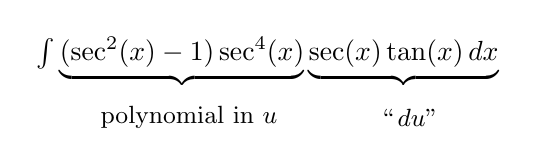
\begin{tikzpicture}
        \node at (0,0) {
          $\int \underbrace{(\sec^2(x)-1)\sec^4(x)} \underbrace{\sec(x)\tan(x) \d x}$
        };
        \node at (-1,-.7) {\small{polynomial in $u$}};
        \node at (1.8,-.7) {\small{``$\d u$''}};
      \end{tikzpicture}
    \end{center}
    Making the substitution
    \begin{align*}
      u &= \sec(x)\\
      \d u &=\answer[given]{\sec(x)\tan(x)} \d x
    \end{align*}
    yields
    \[
    \int \answer[given]{(u^2-1)u^4} \d u
    \]
    This is a polynomial in $u$, and so we can easily finish the
    integration by just expanding the polynomial out and integrating
    term-by-term. We leave it to the interested mathematician to
    finish this problem.
  \end{explanation}
\end{example}

%Again we can generalize the pattern in the previous problem. In order for the previous method to succeed we needed to the integrand to be a product of powers 
%of $\tan(x)$ and $\sec(x)$ where the power of $\tan(x)$ is odd. 
%
%\[
%\int \tan^{2k-1}(x) \sec^{m}(x) \d x
%\]
%
%
%We can then pull out a $\sec(x)\tan(x)$ factor to get 
%
%\[
%\int \tan^{2k}(x) \sec^{m-1}(x) \sec(x)\tan(x) \d x
%\]
%
%Now we can rewrite the $\tan^{2k}(x)$ as the power of a square:
%
%\[
%\int (\tan^{2}(x))^{k} \sec^{m-1}(x) \sec(x)\tan(x) \d x
%\]
%
%We use the identity $\tan^{2}(x)=\sec^{2}(x)-1$ to express the $\tan^{2}(x)$ factor
%
%\[
%\int (\sec^{2}(x)-1)^{k} \sec^{m-1}(x) \sec(x)\tan(x) \d x
%\]
%
%Now we do the substitution $u=\sec(x)$ and $\d u=\sec(x)\tan(x)$. 
%
%\[
%\int (u^{2}-1)^{k} u^{m-1} \d u
%\]
%
%Yet again we have produced a polynomial in $u$ which can, in principle, be expanded and integrated term by term. 


%%%%%POSSIBLY ADD BACK???%%%%%%%%%%%%


%\subsection{Powers of cosecant and cotangent}
%
%Integrals involving powers of $\cot(x)$ and $\csc(x)$ work in a similar fashion to those involving $\tan(x)$ and $\sec(x)$. The $\cot(x)$ 
%plays a role similar to $\tan(x)$ while $\csc(x)$ plays a role similar to $\sec(x)$. For completeness, we do two examples to illustrate the idea.
%
%\begin{example}
%  Compute
%  \[
%  \int \cot^3(x) \csc^4(x) \d x
%  \]
%  \begin{explanation}
%    Notice that the power of $\csc(x)$ is even. Treating it just like an integral with an even power of $\sec(x)$ from 
%    the previous section, we pull out a $\csc^{2}(x)$ term. 
%    \begin{align*}
%      \int &\cot^3(x) \csc^4(x) \d x \\
%    &= \int\cot^3(x) \csc^2(x) \csc^2(x) \d x
%    \end{align*}
%    Now using the Pythagorean identity $\csc^{2}(x)=1+\cot^{2}(x)$, we can rewrite everything in
%    terms of $\cot(x)$, but reserve the one power of $\csc^2(x)$ to use for the differential in an eventual variable substitution $u=\cot(x)$:
%    \begin{center}%% used center instead of image since there is no reason for a LARGE integral in the text
%      \begin{tikzpicture}
%        \node at (0,0) {
%          $\int \underbrace{(\cot^3(x)(\cot^2(x)+1)} \underbrace{\csc^2(x) \d x}$
%        };
%        \node at (-.5,-.7) {\small{polynomial in $u$}};
%        \node at (1.8,-.7) {\small{``$\d u$''}};
%      \end{tikzpicture}
%    \end{center}
%    Making the substitution
%    \begin{align*}
%      u &= \cot(x)\\
%      \d u &=\answer[given]{-\csc^2(x)} \d x
%    \end{align*}
%    yields
%    \[
%    \int \answer[given]{-u^3(u^2+1)} \d u
%    \]
%    This is a polynomial in $u$, and so we can easily finish the
%    integration by just expanding the polynomial out and integrating
%    term-by-term. We leave it to the fearless mathematician to
%    finish this problem.
%  \end{explanation}
%\end{example}
%
%
%
%
%\begin{example}
%  Compute
%  \[
%  \int \cot^3(x) \csc^5(x) \d x
%  \]
%  \begin{explanation}
%     The power of $\csc(x)$ is not even but the power of $\cot(x)$ is odd. Mirroring the strategy we used in the 
%case of a product of an odd power of $\cot(x)$ with an odd power of $\csc(x)$, we pull out a 
%   $\csc(x)\cot(x)$ term to use for the differential. 
%    \begin{align*}
%      \int &\cot^3(x) \csc^5(x) \d x \\
%    &= \int\cot^2(x) \csc^4(x) \csc(x)\cot(x) \d x
%    \end{align*}
%    Now using the Pythagorean identity$ \cot^{2}(x)=\csc^{2}(x)-1$ we can rewrite everything in
%    terms of $\csc(x)$, but reserving the one power of $\csc(x)\cot(x)$ to help
%    with the differential in an eventual variable substitution $u=\csc(x)$:
%    \begin{center}%% used center instead of image since there is no reason for a LARGE integral in the text
%      \begin{tikzpicture}
%        \node at (0,0) {
%          $\int \underbrace{(\csc^2(x)-1)\csc^4(x)} \underbrace{\csc(x)\cot(x) \d x}$
%        };
%        \node at (-1,-.7) {\small{polynomial in $u$}};
%        \node at (1.8,-.7) {\small{``$\d u$''}};
%      \end{tikzpicture}
%    \end{center}
%    Making the substitution
%    \begin{align*}
%      u &= \csc(x)\\
%      \d u &=\answer[given]{-\csc(x)\cot(x)} \d x
%    \end{align*}
%    yields
%    \[
%    \int \answer[given]{-(u^2-1)u^4} \d u
%    \]
%    This is a polynomial in $u$, and so we can easily finish the
%    integration by just expanding the polynomial out and integrating
%    term-by-term. We leave it to the patient young mathematician to
%    finish this problem.
%  \end{explanation}
%\end{example}
%
%
%
%
%
%
%
%
%
There is no analogue for the power reduction formulas for sines and cosines, so sometimes, these integrals can become a bit trickier.

\begin{example}
Compute: 
\[
\int \sec^{4}(x) \d x 
\]
\begin{explanation}
 There are no powers of $\tan(x)$ immediately available here, so letting $u=\tan(x)$ may seem like a bad idea at first.  However, by saving a copy of $\sec^2(x)$ for the differential, we have $2$ powers of $\sec(x)$ left, so let's give it a try:
 
    \begin{align*}
    \int \sec^{4}(x) \d x  &= \int \sec^2(x) \sec^2(x) \d x
    \end{align*}
    Now using the identity $\sec^{2}(x)=\tan^{2}(x)+1$ we can write:
    \begin{center}%% used center instead of image since there is no reason for a LARGE integral in the text
      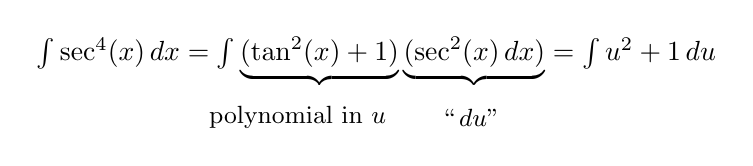
\begin{tikzpicture}
        \node at (0,0) {
          $\int \sec^{4}(x) \d x  =  \int  \underbrace{(\tan^2(x)+1)} \underbrace{(\sec^2(x) \d x)} = \int u^2+1 \d u$
        };
        \node at (-1,-.7) {\small{polynomial in $u$}};
        \node at (1.2,-.7) {\small{``$\d u$''}};
      \end{tikzpicture}
    \end{center}
   
   Integrating this, we find:
   
   \begin{align*}
   \int \sec^{4}(x) \d x  &= \frac{1}{3}u^3+u +C\\
   &= \frac{1}{3} \tan^3(x)+\tan(x)+C
   \end{align*}
\end{explanation}
\end{example} 

\begin{example}
Compute: 
\[
\int \sec^{3}(x) \d x 
\]
\begin{explanation}
Our previous techniques for handling powers of $\sec(x)$ and $\tan(x)$ relied on having an even power of $\sec(x)$ or an odd power of $\tan(x)$. 
Suppose we split off a $\sec^{2}(x)$ to write the integral as 
\[
 \int \sec(x) \sec^{2}(x) \d x
\]
The $\sec^{2}(x)$ is the antiderivative of $\tan(x)$ but there is no $\tan(x)$ term so $u$ substitution will not work. Since we have a product of two functions where one 
of the functions can be easily integrated let's try integration by parts. 

Choose
\[ 
u= \sec(x) \text{  and  } \d v=\sec^{2}(x) \\
\] 
\[
\d u=  \sec(x)\tan(x) \d x \text{  and  } v=\tan(x) 
\]

We recall the integration by parts formula $\int u \d v=uv-\int v \d u$, so we obtain

\[
\int \sec^{3}(x) \d x=\sec(x)\tan(x) - \int \tan^{2}(x)\sec(x)\d x
\]

The rightmost integral does not have an odd power of $\tan(x)$ or an even power of $\sec(x)$ but we could convert 
everything to be in terms of $\sec(x)$ by using the identity $\tan^{2}(x)=\sec^{2}(x)-1$. 

The rightmost integral then becomes
\[
\int \tan^{2}(x)\sec(x) \d x=\int (\sec^{2}(x)-1) \sec(x) \d x= \int \sec^{3}(x)\d x - \int \sec(x) \d x
\]

Combining this with our original integral and using the previous example which gave us $\int \sec(x) \d x$ we get
\[
\int \sec^{3} \d x=\sec(x) \tan(x)- \int \sec^{3} \d x + \ln| \sec(x)+\tan(x) | + C
\]

Notice that the remaining integral on the right hand side is simply the original integral we were trying to determine. You will remember that we first experienced this phenomenon in the section on integration by parts when we tried to compute $\int e^{x}\cos(x) \d x$. 
Since the desired unknown quantity appears on the left and the right we simply solve for it and so

\[
\int \sec^{3}(x) \d x=\frac{1}{2}\left(\sec(x) \tan(x) + \ln | \sec(x) + \tan(x)|  \right)  + C
\]
\end{explanation}
\end{example}

This last example can be generalized to a reduction formula for $\int \sec^{n}(x) \d x$. We omit the details but using integration by parts in a similar fashion
as above with $u=\sec^{n-2}(x)$ and $\d v=\sec^{2}(x)$ gives us the following reduction formula:

\[
\int \sec^{n}(x) \d x= \frac{\tan(x) \sec^{n-2}(x)}{n-1} + \frac{n-2}{n-1} \int \sec^{n-2}(x) \d x 
\]

We won't derive them here but note that there are similar reduction formulas that we could derive for integrating powers of other trigonometric functions using integration by parts. 

%The example of $\int \sec^{3}(x) \d x$ as well as $\int \sec^{n}(x) \d x$ gives us one possible strategy to handle integrals that involve powers of $\tan(x)$ and $\sec(x)$ 
%where the power of $\tan(x)$ is even and the power of $\sec(x)$ is odd. 
%
%
%The idea is to write the even power of $\tan(x)$ in terms of $\sec(x)$ using 
%\[ 
%\tan^{2}(x)=\sec^{2}(x)-1
%\]
%
%The result will be a polynomial in $\sec(x)$. 
%One can then use integral properties to break the integral up into a sum of integrals involving powers of $\sec(x)$ which can then be integrated using 
%the above reduction formula.  
%
%
%Note!: For many trigonometric integrals of the type we have examined in this section, there may be several techniques which apply to allow us to 
%determine the antiderivative.
%Consider the example
%\[
%\int \tan^{3}(x) \sec^{4}(x) \d x 
%\]
%that occured earlier in the text. When we first encountered this example, we split off a $\sec^{2}(x)$ and 
%converted the leftover $\sec^{2}(x)$ term 
%\[
%\int \tan^{3}(x) (1+\tan^{2}(x)) \sec^{2}(x) \d x
%\]
%
%We then did the substitution $u=\tan(x)$ to convert the integrand to be a polynomial in $u$. 
%
%Another possible strategy is to notice that the power of $\tan(x)$ is odd.  We can then use the substitution $u=sec(x)$ after pulling out a $\sec(x)\tan(x)$ term and converting 
%$\tan^2(x)$ to be in terms of $\sec(x)$. 
%
%\[
%\int (\sec^{2}(x)-1) \sec^{3}(x) \sec(x)\tan(x) \d x
%\]
%We then do the substitution $u=\sec(x)$ to convert the integrand to be a polynomial in $u$. 
%
%In fact there is third strategy that we can use. We  can convert the integrand to be in terms of $\sin(x)$ and $\cos(x)$. 
%
%We get 
%\[
%\int \frac{\sin^{3}(x)}{\cos^{7 }(x) } \d x
%\]
%
%Here the power of $\sin(x)$ is odd so we can separate off a $\sin(x)$ to be used for $\d u$ and convert
%the remaining even power of $\sin(x)$ using $\sin^{2}(x)=1-\cos^{2}(x)$. 
%
%\[
%\int \frac{(1-\cos^{2}(x)) \sin(x)}{\cos^{7}(x) } \d x
%\]
%The substitution $u=\cos(x)$ then converts this integral into a rational function of $u$ which can be simplified and integrated 
%term by term. 
\begin{remark}
Note, it is also possible to run across trigonometric integrals where none of these techniques immediately apply.  If all else fails, one strategy is to convert all trigonometric functions to sines and cosines.
\end{remark}

\begin{remark}
The same strategies can be employed to work with integrals involving powers of cosecants and cotangents since both the Pythagorean identities and the derivatives of these functions behave analogously to those for tangents and secants.
\end{remark}


\section{Final thoughts}

When we encounter integrals that involve products of complimentary trigonometric functions (sines and cosines, tangents and secants, or cosecants and cotangents), we can employ a general strategy to find the antiderivatives:

\begin{itemize}
\item Let $u$ be one of the trigonometric functions.  Peel off a copy of the derivative for the differential.  If this leaves an even number of the other trigonometric function, use the appropriate Pythagorean identity to write the remaining powers of the other trigonometric function in terms of $u$.  
\item If the integral involves a product of sines and cosines and the above does not work, try using the power reduction formulas.
\item If the integral involves secants and tangents (or cosecants and cotangents), try either integration by parts or convert everything to sines and cosines.
\end{itemize}

As usual, practice is necessary to develop good intuition when working these types of problems.

\begin{quote}
``One should study mathematics simply because it helps to arrange one's ideas" - M. W. Lomonossow
\end{quote}









\end{document}

